\chapter{روش‌شناسی تحقیق}\label{Chap:chap3}
{}

\section{مقدمه}

در این فصل، روش‌شناسی پژوهش و مراحل انجام کار به منظور طراحی و پیاده‌سازی سامانه‌ی پرسش و پاسخ هوشمند در حوزه‌ی اورولوژی شرح داده می‌شود. ابتدا معماری کلی سامانه معرفی می‌گردد. سپس روش گردآوری و آماده‌سازی داده‌ها، ابزارها و فناوری‌های مورد استفاده و در نهایت، روش ارزیابی سامانه تشریح می‌گردد.

\section{معماری کلی سامانه}

معماری سامانه بر اساس الگوی خط‌لوله داده
\LTRfootnote{Data pipeline}
طراحی شده است. این معماری از شش مؤلفه اصلی تشکیل می‌شود که در شکل \ref{fig:architecture} نمایش داده شده است.
\begin{figure}[ht]
\centerline{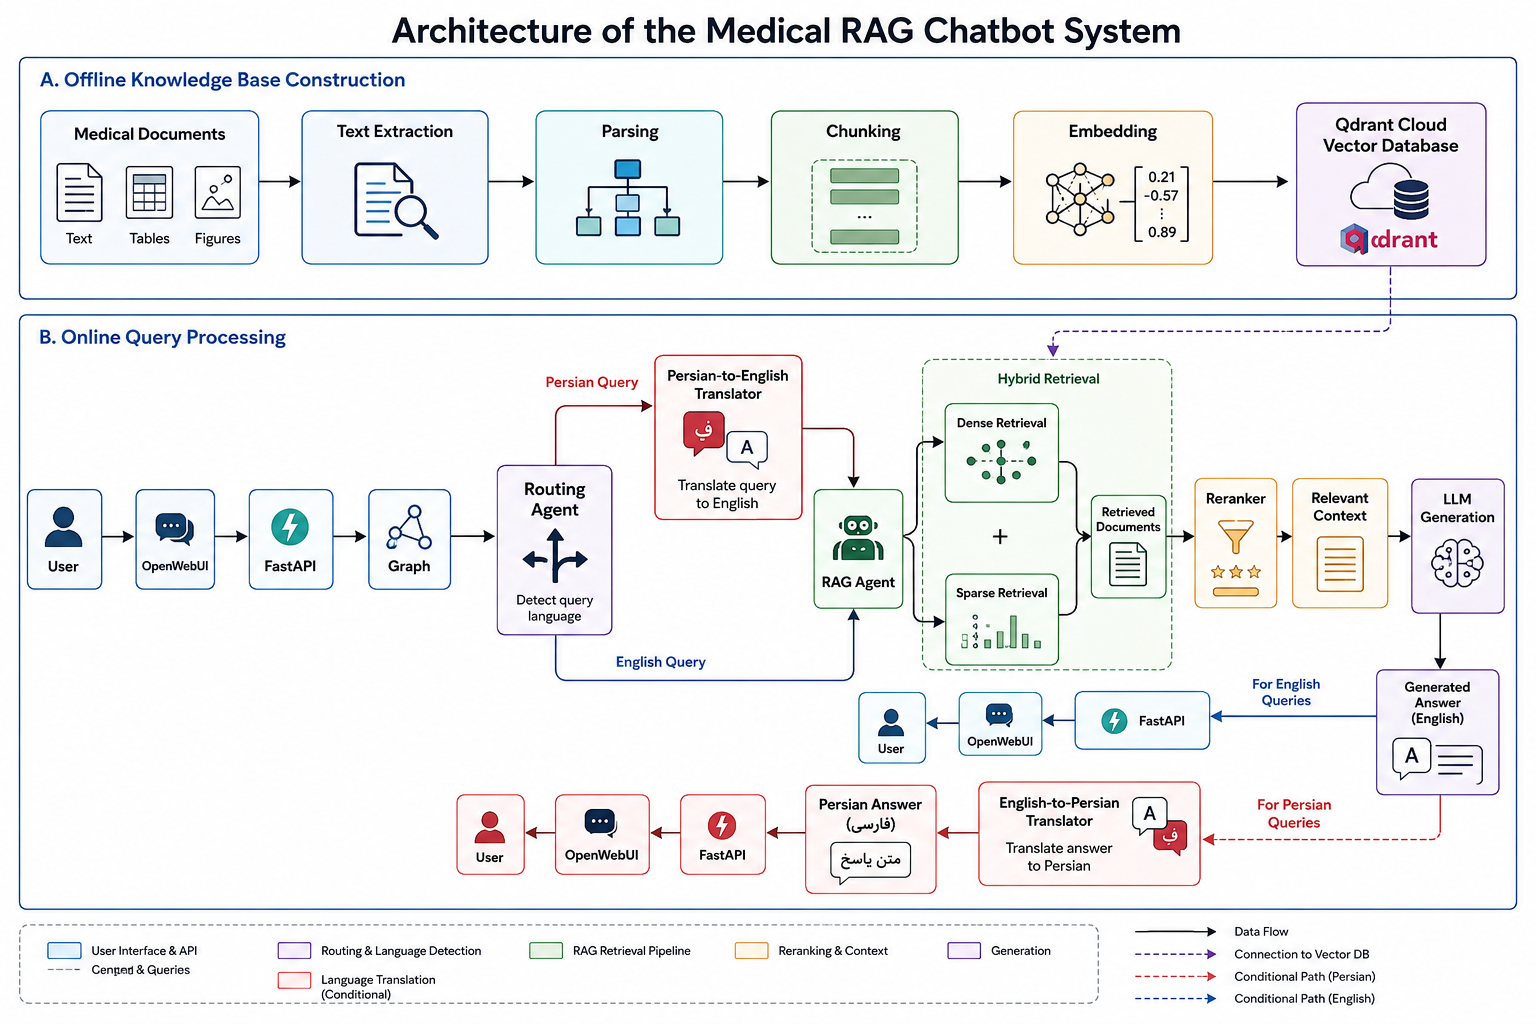
\includegraphics[width=8cm]{architecture.png}}
\caption{معماری کلی سامانه‌ی پیشنهادی}
\label{fig:architecture}
\end{figure}

همان‌گونه که در شکل \ref{fig:architecture} مشاهده می‌شود، جریان داده در سامانه به صورت زیر است:


\begin{enumerate}
\item کاربر پرسش خود را از طریق رابط کاربری وارد می‌کند.
\item عامل مسیر‌یابی
\LTRfootnote{Router Agent}، زبان پرسش را تشخیص می‌دهد. در صورتی که پرسش به زبان فارسی باشد، به عامل ترجمه هدایت می‌گردد.
\item عامل ترجمه
\LTRfootnote{Translator Agent}، پرسش را به زبان انگلیسی ترجمه می‌کند.
\item موتور بازیابی
\LTRfootnote{Retriever}، قطعات مرتبط را از پایگاه داده‌ی برداری بازیابی می‌نماید.
\item موتور باز‌رتبه‌بندی
\LTRfootnote{Re-ranker}، قطعات بازیابی‌شده را به ترتیب اهمیت مرتب می‌کند.
\item مدل زبانی
\LTRfootnote{Large Language Model}، پاسخ نهایی را بر اساس پرسش و قطعات مرتب‌شده تولید می‌کند.
\item پاسخ تولیدشده، در صورت نیاز به فارسی ترجمه شده و به کاربر نمایش داده می‌شود.
\end{enumerate}


\section{داده‌های مورد استفاده}

داده‌های مورد استفاده این پژوهش، شامل متون پزشکی مرتبط با حوزه‌ی اورولوژی است. این متون شامل موارد زیر هستند:

\begin{itemize}
\item کتاب کمپبل-والش اورولوژی، چاپ سیزدهم
\LTRfootnote{Campbell-Walsh Urology, 13th Edition}
\item کتاب اسمیت و تاناگوس اورولوژی عمومی، چاپ نوزدهم
\LTRfootnote{Smith and Tanaghos General Urology, 19th Edition}
\item راهنمای بالینی انجمن اورولوژی اروپا (۲۰۲۶)
\LTRfootnote{EAU Guidelines 2026}
\end{itemize}

\section{روش گردآوری و آماده‌سازی داده‌ها}

داده‌ها با استفاده از روش‌های زیر گردآوری شده‌اند: تهیه‌ی نسخه‌ی الکترونیکی منابع، تبدیل فایل‌های PDF به متن قابل پردازش، و تفکیک محتوای هر کتاب بر اساس فصل‌ها و بخش‌های اصلی.

\subsection{استخراج متون داده‌ها}

متون کتاب‌ها با استفاده از کتابخانه‌ی پی‌ام‌یو‌پی‌دی‌اف۴ال‌ال‌ام
\LTRfootnote{pymupdf4llm} استخراج می‌شوند.

\subsection{پاک‌سازی داده}

در این گام کاراکترهای اضافی، فاصله‌های بی‌رویه و علائم غیراستاندارد از متن حذف می‌شوند. همچنین برای تصاویر و نمودار‌های مهم متون توصیفی تهیه می‌گردد. سرفصل‌ها با استفاده از علائم در متن مشخص می‌گردند تا در ادامه در استخراج فراداده مورد استفاده قرار بگیرند.

\subsection{قطعه‌بندی}

قطعه‌بندی در دو مرحله انجام می‌پذیرد. مرحله اول هر فصل کتاب به یک قطعه تبدیل می‌گردد و در مرحله دوم هر فصل به تعدادی زیر قطعه تقسیم شد. اندازه‌ی هر قطعه ۱۰۰۰ توکن و میزان همپوشانی ۲۰۰ توکن است. شایان ذکر است که حداقل اندازه‌ی هر قطعه، ۱۵۰ توکن در نظر گرفته شده است. این امر به منظور جلوگیری از تولید قطعات بسیار کوچک که صرفاً شامل سرفصل‌ها یا اطلاعات ناقص هستند، انجام می‌پذیرد.

\subsection{استخراج فراداده}

برای هر قطعه، فراداده‌های زیر استخراج و ذخیره می‌شوند:

\begin{itemize}
\item شناسه قطعه
\item شناسه قطعه پدر
\item شماره قطعه
\item نام مرجع
\item نام مرجع همراه با شماره و نام فصل
\item متن قطعه
\item شناسه‌ای برای تعیین اینکه این قطعه دارای جدول هست یا خیر
\end{itemize}


\section{ابزارها و فناوری‌های مورد استفاده}

ابزارها و فناوری‌های به کار رفته در این پژوهش در جدول \eqref{tab:tools} معرفی شده‌اند.

\begin{table}[ht]
\caption{ابزارها و فناوری‌های مورد استفاده}
\label{tab:tools}
\centering
\onehalfspacing
\begin{tabular}{|c|c|c|}
\hline
\textbf{ابزار} & \textbf{کاربرد} & \textbf{نسخه} \\
\hline
پایتون (Python) & زبان برنامه‌نویسی اصلی & 3.11 \\
\hline
کوانت (Qdrant) & پایگاه داده‌ی برداری & ۰.۴.۲۲ \\
\hline
فست‌ای‌پی‌آی (FastAPI) & پیاده‌سازی API & ۰.۱۰۰.۰ \\
\hline
جی‌پی‌تی-۴ (GPT-4) & مدل زبانی برای تولید پاسخ & ۰۶۱۳ \\
\hline
ان‌ال‌ال‌بی-۲۰۰ (NLLB-200) & مدل ترجمه & ۳.۳ میلیارد پارامتر \\
\hline
داکر (Docker) & ظرفی‌سازی سامانه & ۲۰.۱۰ \\
\hline
\end{tabular} 
\end{table}


\section{روش ارزیابی سامانه}

به منظور ارزیابی عملکرد سامانه‌ی طراحی‌شده، عملکرد آن در دو سطح
بازیابی اطلاعات و تولید پاسخ مورد بررسی قرار می‌گیرد. در سطح
بازیابی، میزان ارتباط قطعات متنی بازیابی‌شده با پرسش ارزیابی شده
و عملکرد روش بازیابی ترکیبی و مرحله‌ی بازرتبه‌بندی مورد بررسی قرار
می‌گیرد. در سطح تولید پاسخ نیز کیفیت پاسخ نهایی سامانه از نظر
صحت، ارتباط با پرسش و میزان انطباق با اطلاعات بازیابی‌شده ارزیابی
می‌شود.

\subsection{مجموعه‌داده ارزیابی}


برای ارزیابی عملکرد سامانه، از یک مجموعه‌داده شامل ۲۰۲ پرسش
چندگزینه‌ای در حوزه‌ی اورولوژی استفاده می‌شود. هر پرسش شامل متن
سؤال، گزینه‌های پاسخ و پاسخ صحیح به همراه توضیح مربوط به آن است.
پرسش‌ها به عنوان ورودی بخش بازیابی به سامانه داده می‌شوند و قطعات متنی
مرتبط از پایگاه داده‌ی برداری بازیابی می‌گردند

\subsection{ارزیابی بخش بازیابی}


برای ارزیابی بخش بازیابی، پرسش‌ها به سامانه‌ی Hybrid Retrieval
داده شده و برای هر پرسش، تعدادی از مرتبط‌ترین قطعات متنی از
پایگاه داده‌ی برداری بازیابی می‌شوند. در روش پیشنهادی، بازیابی
اطلاعات با استفاده از ترکیب نتایج بازیابی متراکم و تنک و ادغام
آن‌ها با روش Reciprocal Rank Fusion (RRF) انجام می‌شود.

به منظور تعیین میزان ارتباط قطعات بازیابی‌شده با هر پرسش، از یک
مدل زبانی به عنوان ارزیاب استفاده می‌شود. این مدل، میزان ارتباط
هر قطعه با پرسش را در مقیاسی از صفر تا چهار تعیین می‌کند. امتیاز
صفر نشان‌دهنده‌ی عدم ارتباط قطعه با پرسش و امتیاز چهار نشان‌دهنده‌ی
ارتباط مستقیم و کافی قطعه برای پاسخ‌گویی به پرسش است. در این
ارزیابی، قطعات دارای امتیاز ۳ یا ۴ به عنوان قطعات مرتبط در نظر
گرفته می‌شوند.

\subsection{معیارهای ارزیابی بازیابی}


برای سنجش عملکرد بخش بازیابی، معیارهای زیر مورد استفاده قرار
می‌گیرند:


\begin{itemize}

\item \textbf{نرخ برخورد در موقعیت K (Hit@K)}
\LTRfootnote{Hit@K}:
این معیار مشخص می‌کند که آیا حداقل یک قطعه‌ی مرتبط با پرسش در میان
$K$ نتیجه‌ی اول بازیابی‌شده قرار گرفته است یا خیر. مقدار این معیار
از نسبت تعداد پرسش‌هایی که حداقل یک قطعه‌ی مرتبط در میان $K$ نتیجه‌ی
اول آن‌ها قرار دارد به تعداد کل پرسش‌ها به دست می‌آید.

\item \textbf{میانگین ارتباط در موقعیت K (Mean Relevance@K)}
\LTRfootnote{Mean Relevance@K}:
این معیار میانگین امتیاز ارتباط قطعات موجود در میان $K$ نتیجه‌ی
اول را نشان می‌دهد و برای بررسی میزان ارتباط نتایج بازیابی‌شده
با پرسش مورد استفاده قرار می‌گیرد.

\end{itemize}


به منظور بررسی عملکرد سامانه در رتبه‌های مختلف، معیارهای مذکور
برای مقادیر مختلف $K$ شامل $1$، $3$، $5$ و $10$ محاسبه می‌شوند.


\subsection{ارزیابی اثر بازرتبه‌بندی}


با توجه به استفاده از یک مرحله‌ی بازرتبه‌بندی
\LTRfootnote{Reranking} پس از بازیابی اولیه، عملکرد نتایج قبل و بعد
از بازرتبه‌بندی به صورت جداگانه ارزیابی می‌شود. در این مرحله،
نتایج اولیه‌ی حاصل از \LTRfootnote{Hybrid Retrieval} به عنوان ورودی بازرتبه‌بند
در نظر گرفته شده و پس از تعیین مجدد ترتیب نتایج، عملکرد مجموعه‌ی
بازرتبه‌بندی‌شده با نتایج اولیه مقایسه می‌شود.

برای این منظور، معیارهای Hit@K و Mean Relevance@K پیش و پس از
بازرتبه‌بندی محاسبه و مقایسه می‌شوند. این مقایسه امکان بررسی تأثیر
مرحله‌ی بازرتبه‌بندی بر بهبود جایگاه قطعات مرتبط و انتخاب اطلاعات
مناسب‌تر برای مرحله‌ی تولید پاسخ را فراهم می‌کند.


\subsection{ارزیابی زمان پاسخ‌دهی}


علاوه بر کیفیت بازیابی و پاسخ، زمان اجرای سامانه نیز مورد بررسی
قرار می‌گیرد. برای این منظور، زمان مورد نیاز برای پردازش یک پرسش
از مرحله‌ی دریافت ورودی تا تولید پاسخ نهایی اندازه‌گیری شده و
میانگین زمان پاسخ‌دهی در مجموعه‌ی آزمون گزارش می‌گردد


\subsection{ارزیابی کیفی پاسخ‌های تولیدشده}


در کنار معیارهای کمی، نمونه‌هایی از پاسخ‌های تولیدشده توسط سامانه
به صورت کیفی بررسی می‌شوند. در این بررسی، میزان انطباق پاسخ با
اطلاعات موجود در منابع بازیابی‌شده، صحت محتوای پاسخ، ارتباط پاسخ
با پرسش و میزان استفاده‌ی صحیح از اطلاعات بازیابی‌شده مورد توجه
قرار می‌گیرد.

همچنین عملکرد سامانه در شرایطی که اطلاعات کافی برای پاسخ‌گویی در
منابع موجود نیست، بررسی می‌شود تا مشخص شود سامانه از تولید پاسخ
بدون پشتوانه‌ی کافی جلوگیری می‌کند.


\subsection{معیارهای ارزیابی کیفی}

پاسخ‌های تولیدشده توسط سامانه، توسط متخصصین حوزه‌ی اورولوژی از جنبه‌های زیر و در مقیاس ۱ تا ۵ امتیازدهی می‌شوند:

\begin{itemize}

\item \textbf{دقت بالینی}: میزان صحت اطلاعات پزشکی ارائه‌شده در پاسخ؛

\item \textbf{جامعیت}: میزان پوشش مناسب جنبه‌های مورد انتظار در پاسخ
به پرسش؛

\item \textbf{قابلیت استناد}: میزان پشتیبانی پاسخ از اطلاعات موجود
در منابع بازیابی‌شده و صحت ارجاعات ارائه‌شده؛

\item \textbf{قابلیت فهم}: میزان وضوح و قابل‌درک بودن پاسخ برای
مخاطب مورد نظر.

\end{itemize}


\section{جمع‌بندی}

در این فصل، روش‌شناسی پژوهش شامل معماری کلی، روش گردآوری و آماده‌سازی داده‌ها، ابزارهای مورد استفاده و روش ارزیابی تشریح گردید. در فصل چهارم، جزئیات پیاده‌سازی مؤلفه‌های مختلف سامانه و نتایج حاصل از ارزیابی ارائه خواهد شد.
